\DeclarePairedDelimiter\abs{\lvert}{\rvert}%
\begin{frame}{Saturating Functions}
	\begin{itemize}
		\item A saturating activation function squeezes the input.
		\begin{align*}
			(\abs{\lim_{x \to -\infty}f(x)}=+\infty)
			\vee (\abs{\lim_{x \to +\infty}f(x)}=+\infty)
		\end{align*}
		\begin{figure}[H]
			\centering
			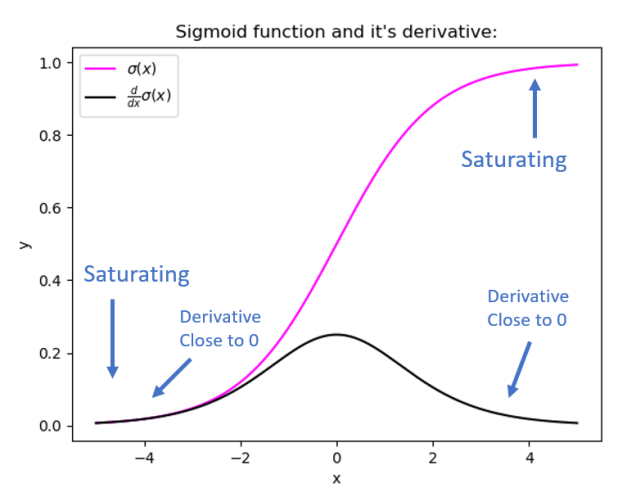
\includegraphics[width=0.5\textwidth]{Figs/van_1.png}
			\caption{Saturating Functions, \href{https://www.analyticsvidhya.com/blog/2021/06/the-challenge-of-vanishing-exploding-gradients-in-deep-neural-networks/}{Source}}
		\end{figure}
	\end{itemize}
\end{frame}

\begin{frame}{Saturating Functions}
	\begin{itemize}
		\item The Tanh (hyperbolic tangent) activation function is saturating as it squashes real numbers to range between $(-1, 1)$
	\end{itemize}
	\begin{figure}[H]
		\centering
		\resizebox{0.45\textwidth}{!}{
			\begin{tikzpicture}
				\begin{axis} [axis lines=middle]
					\addplot [color=red, domain=-10:10, smooth, thick] {(exp(x)-exp(-x))/(exp(x)+exp(-x))};
				\end{axis}
		\end{tikzpicture}}
		\caption{Hyperbolic Tangent}
	\end{figure}
\end{frame}

\begin{frame}{Saturating Functions}
	\begin{itemize}
		\item The Sigmoid activation function  $f(x) = \frac{1}{1+\exp^{-x}}$ is also saturating, because it squashes real numbers to range between $(0, 1)$.
	\end{itemize}
	\begin{figure}[H]
		\centering
		\resizebox{0.45\textwidth}{!}{
		\begin{tikzpicture}
			\begin{axis} [axis lines=middle]
				\addplot [color=red, domain=-6:6, smooth, thick] {1/(1+exp(-x))};
			\end{axis}
		\end{tikzpicture}}
		\caption{Sigmoid}
	\end{figure}
\end{frame}

\begin{frame}{Saturating Functions}
	\begin{itemize}
		\item In contrast, The Rectified Linear Unit (ReLU) activation function is non-saturating.
	\end{itemize}
	\begin{figure}[H]
		\centering
		\resizebox{0.6\textwidth}{!}{
			\begin{tikzpicture}
				\begin{axis} [axis lines=middle, unit vector ratio*=1 1 1]
					\addplot [color=red, domain=-10:0, smooth, very thick] {0};
					\addplot [color=red, domain=0:10, smooth, thick] {x};	
				\end{axis}
		\end{tikzpicture}}
		\caption{ReLU}
	\end{figure}
\end{frame}

